\section{Digitalisation in practice}

The workshop started with presentations by three groups that have all been exploring digitalisation of wind lidar. Summaries for each presenation were provided by the presenters.

\subsection{How the common lidar data format improved our data processing (Ines Würth)}

\begin{altquote}
    In 2018 DTU, Fraunhofer IEE and others published the report from their e-WindLidar project \citep{nikola_vasiljevic_2018_2478051} in which they introduced a common format for wind lidars. Up to now, lidars from different manufacturers spit out data in different formats using different variables. In Stuttgart we therefore developed different code for each lidar in order to process the data.

    The common format brings only advantages: in Stuttgart we implemented it in our code and now only have one data processing routine for different lidar systems. Collaboration is facilitated because exchange of code and data is very easy. Interfaces where data is exchanged are clearly defined. Therefore we believe that the common data format is the basis for a digitized lidar infrastructure of the future.
\end{altquote}
\altattrib{Ines Würth}

The presentation can be found at \href{https://doi.org/10.5281/zenodo.4629675}{https://doi.org/10.5281/zenodo.4629675} \cite{wurth_ines_2021_4629675}.

\subsection{The Smart Lidar Concept - New Opportunities for the Lidar Community (David Schlipf)}

\begin{altquote}
    We believe that lidar systems will follow the general trend of technology by adapting to their environment and becoming more adjustable. Here, the “smart lidar” concept intends to provide a helpful framework. 

    The smart lidar consists of a reprogrammable lidar device that can be modified or extended by “apps”. A first version of smart lidar was developed as part of the international research and development (R\&D) project between Flensburg University of Applied Sciences, MOLAS and sowento. A commercial lidar has been modified to process third party algorithms which can be directly integrated in common simulation tools for wind turbines, which significantly simplifies the certification of lidar-assisted control applications. In future we anticipate that these apps can be provided by specialists, allowing lidar users and their customers to take advantage of the wide range of experience in the international wind lidar community. 

The presentation shows the main advantages, current advances, and new opportunities for various stakeholders in the lidar community.
\end{altquote}
\altattrib{David Schlipf}

Further details can be found at \href{https://doi.org/10.5281/zenodo.4627168}{https://doi.org/10.5281/zenodo.4627168} \cite{david_schlipf_2021_4627168}. 

\subsection{Modular wind lidar (Andy Clifton)}
\begin{altquote}
Wind lidar are complex devices that are optimised for particular tasks. However, they often contain basically the same modules - power supply, communications, laser source, optics, scanner - that have different properties and capabilities depending on the task. In 2015 a group of Task 32 members came up with the “Open Lidar” concept for modular lidar \citep{clifton_2019_openlidar}, whereby different hardware and software would be combined for different applications. Modular wind lidar have been built in the past but are not commercially available at this time.

The Open Lidar concept has since been applied as a generic, modular architecture for lidar (Figure \ref{fig:modular_lidar}), which is now documented in the \href{http://data.windenergy.dtu.dk/ontologies/view/ontolidar/en/}{Task 32 Wind Lidar Ontology}. This generic architecture with clear definitions in turn enables the development of a “digital twin” for wind lidar - software representations of real-world hardware.

The first wind lidar digital twin - \emph{Qlunc}, designed to quantify the uncertainty of a lidar device - has just been released (DOI: \href{https://doi.org/10.5281/zenodo.4600881}{10.5281/zenodo.4600881}). Qlunc uses the open lidar architecture and defines uncertainty for the hardware components within each module. The uncertainties can then be combined to estimate the uncertainty of line-of-sight wind speed measurements and the total pointing and range uncertainty. This, in turn, can be used as an input to other tools, such as MOCALUM or YADDUM.

Together these tools offer the chance to effectively simulate wind lidar hardware for many different applications, and optimise them before building or deploying them.
\end{altquote}
\altattrib{Andrew Clifton}

\begin{figure*}[!h]
    \centering
    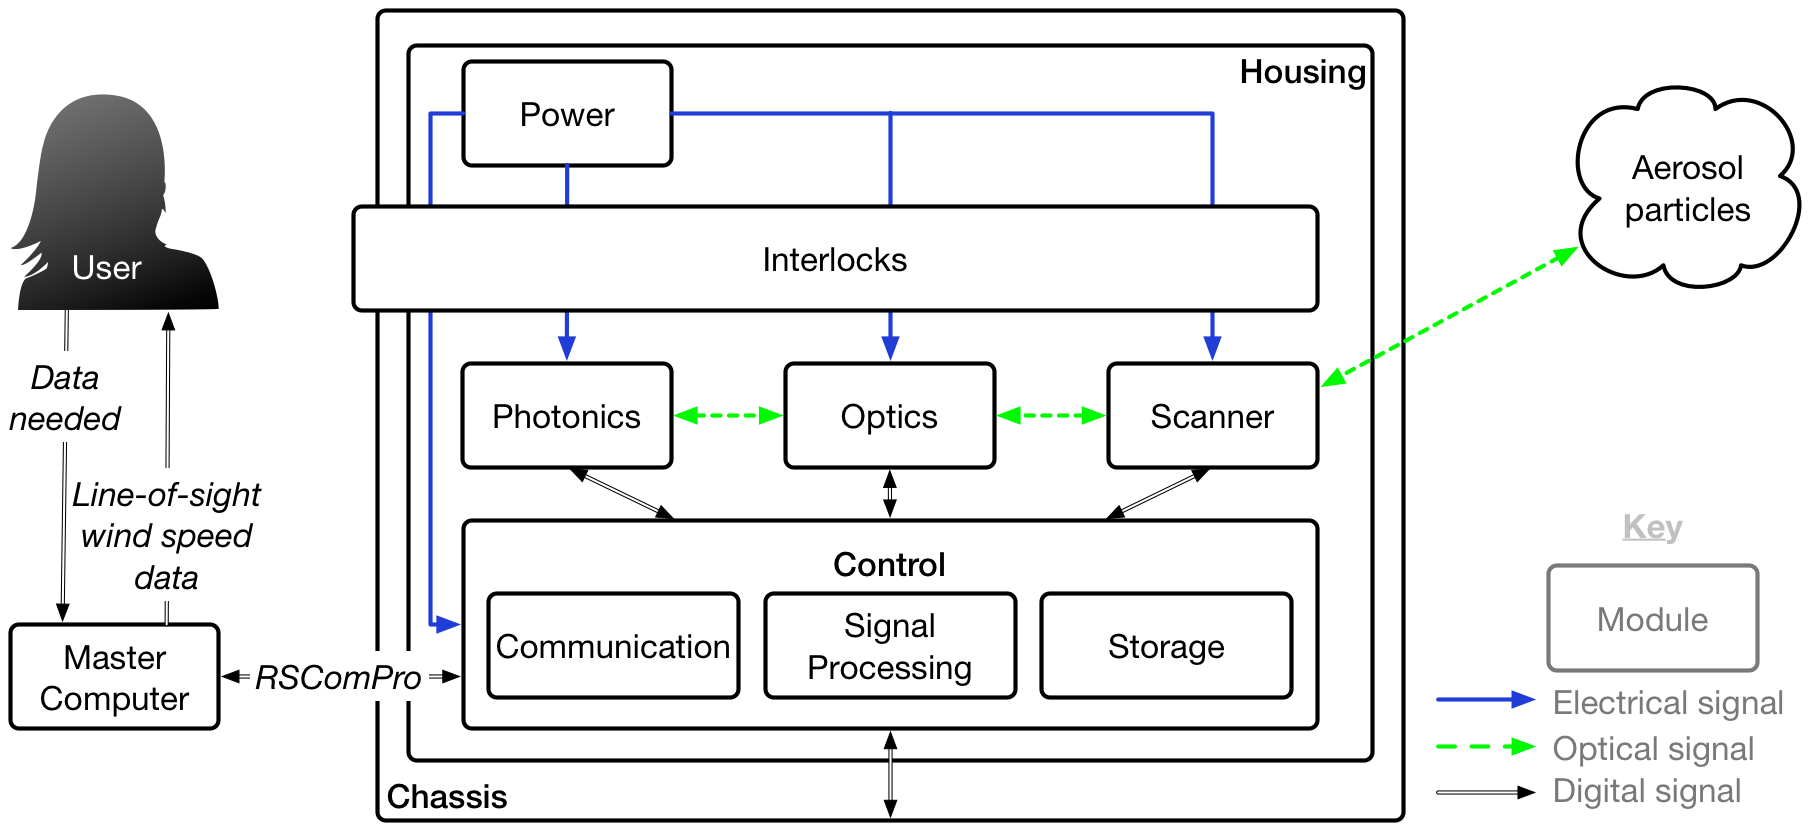
\includegraphics[width=0.85\textwidth]{figures/OpenLidarModules.png}
    \caption{The OpenLidar modular wind lidar architecture \cite{clifton_2019_openlidar}}
    \label{fig:modular_lidar}
\end{figure*}
